\section{Results and Discussion}
\label{sec:results-and-discussion}
% \subsection{Description}
% This section presents the results of your experiments,
% comparing your solution to other schemes. The metrics of
% interest are highly dependent on the topic of research, but
% should optimally cover all interesting aspects of your scheme.
% Informative graphs or tables are the key to a good result
% section.
% Furthermore, you need to discuss your results. You should
% give explanations of distinctive points and outliers in your
% results. It is also necessary to state why your scheme is
% better/worse compared to the other schemes. Thus, this section
% consists of two parts: the results of your experiments, as well
% as an explanation as to why the results are as they are

The speedup associated with each prefetcher for each benchmark, as
well as the average speedup across benchmarks calculated by harmonic
mean, is shown in Figure \ref{fig:comparison}. We test with
prefetching degree varying from $1$ to $7$. For each prefetcher,
numbers for the plot are taken from the degree yielding the highest
average speedup.

The \texttt{ammp} benchmark is noticably more sensitive to different
prefetching strategies than the rest. This indicates that relative to
the other benchmarks, \texttt{ammp} has a memory access pattern more
easily predictable using some methods than others.

\texttt{ammp} and \texttt{wupwise} are the two benchmarks with the
highest speedup.  For the rest, speedup is $1.00\pm0.10$. To better
understand why this is, we look at the accuracy and coverage of the
various prefetchers in Figures \ref{fig:accuracy} and
\ref{fig:coverage}. For most of the benchmarks with low
speedup, either accuracy is low, coverage is low or a combination of
both.

We see that our hybrid prefetcher has lower average speedup than the
simple DC implementation.  By comparing the results in greater detail,
we try to understand why.

\begin{figure*}
  \centering
  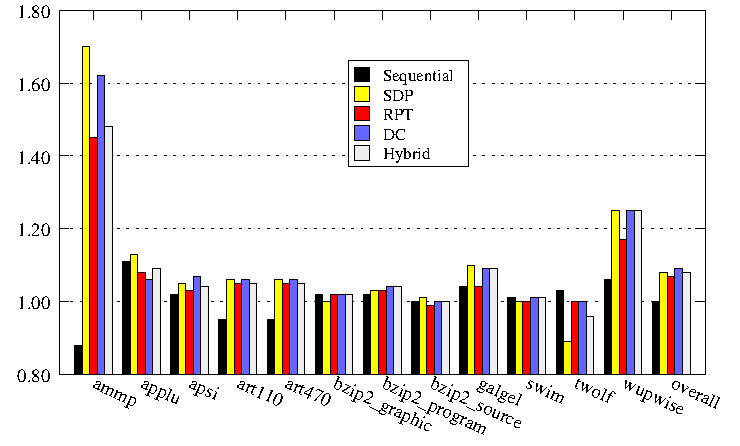
\includegraphics{plots/overview_speedup.pdf}
  \caption{
    Speedup as measured during simulation for each prefetcher grouped by
    benchmark.
    The degree for each prefetcher has been selected to maximize the overall
    performance as measured by the harmonic average displayed to the right.
  }
  \label{fig:comparison}
\end{figure*}

\begin{figure*}
  \centering
  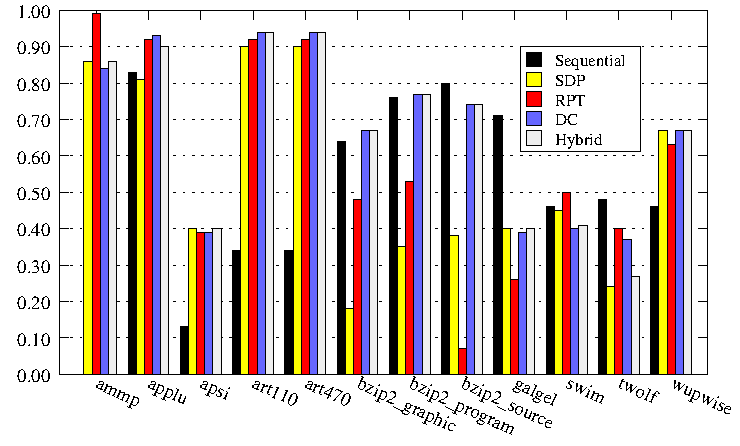
\includegraphics{plots/accuracy_overview.pdf}
  \caption{
      Comparison of prefetcher accuracy for all benchmarks.
      The degrees have been chosen to maximize the harmonic average speedup.
  }
  \label{fig:accuracy}
\end{figure*}

\begin{figure*}
  \centering
  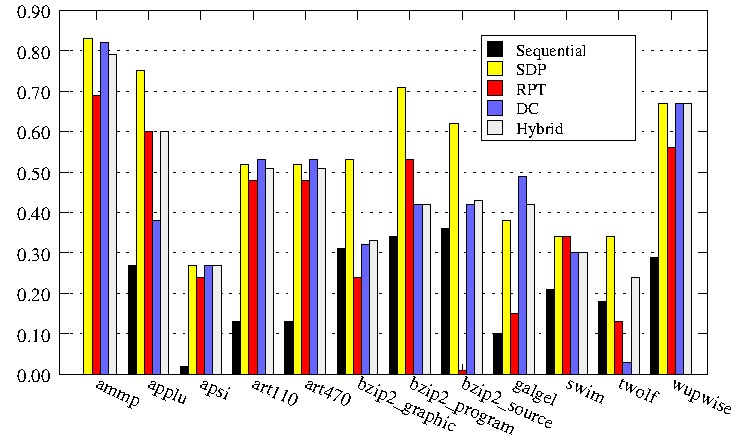
\includegraphics{plots/coverage_overview.pdf}
  \caption{
      Comparison of prefetcher coverage for all benchmarks.
      The degrees have been chosen to maximize the harmonic average speedup.
  }
  \label{fig:coverage}
\end{figure*}


An interesting example showing how the prefetchers differ, is the \texttt{ammp}
benchmark.
This is the benchmark where the performance of the sequential prefetcher is at
its worst;
it degrades performance significantly and a higher prefetching degree only makes
it worse.
Already at degree 1, the accuracy is extremely low at only $0.1\%$, which means
most of the effort put into prefetching blocks is wasted and therefore explains
the low performance.

The SDP prefetcher on the other hand performs quite well and gives a speedup of
$1.7$ for a prefetching degree of $3$.
For this degree, an accuracy of $86\%$ means much fewer of the prefetches are
wasted effort.
As the only difference between this and the sequential prefetcher is the
variable stride used in SDP,
this indicates that the \texttt{ammp} benchmark accesses memory in a linear,
but strided fashion.

The remaining prefetchers all handle strided access and results comparable with
SDP should therefore be expected. 
For delta correlation, the best results are achieved with a prefetching degree
of $6$.
At this degree, $84\%$ of the prefetches turns out to be useful.
The fetches for useless data is probably what makes delta correlation less
effective than SDP despite the improved coverage.
This is also suggested by the $44\%$ increase in average cache miss latency.

For the hybrid prefetcher developed during this project, the speedup on \texttt{ammp} is slightly
worse than for the pure delta correlation approach.
Despite falling back to RPT and eventually SDP, the hybrid approach identifies
fewer prefetches than the delta correlating prefetcher.
Combined with about the same accuracy as for delta correlation, this can explain
the reduced performance.
\todo{Why? It should have more}

Another interesting benchmark is \texttt{wupwise}.
In this benchmark, SDP, delta correlating and hybrid prefetchers all give a
consistent speedup of $1.25$ for all the degrees tested.
RPT is also giving a very consistent speedup of around $1.21$, which is sightly
worse than sequential for degrees greater than 1.
This can be explained if the benchmarks contains long runs of strided memory
access.
Thus the first block after the requested one may not be needed, as assumed in
sequential prefetching, but the next one may be.
As a result, sequential prefetching with a higher degree performs better up to a
certain limit at the maximum stride observed.

Comparing SDP and RPT, both stride based, it becomes clear that the lower
performance of RPT can be explained by a combination of a slightly lower
accuracy and a lower number of identified prefetches.
This may be due to RPT, being more restrictive, only identifies prefetches when
the two last deltas are equal, in contrast to SDP which only requires one.
On the other hand, delta correlation still maintains the same performance while
requiring even more history.
A possible explanation may be that the benchmark's memory access pattern
includes a lot of repeating patterns exploitable by delta correlation.
If the patterns also include some runs of equal deltas, this should be
beneficial to SDP as well because it utilizes shorter runs of equal deltas
better than RPT.

This may also be the reason for the good performance of sequential prefetching
compared to RPT.
From the statistics, RPT only identifies about $72\%$ the number of prefetches
sequential does.
Despite the lower accuracy, this results in a coverage about $15\%$ higher for
sequential.

A noteworthy observation is that the hybrid prefetcher performs comparably to
SDP and delta correlation, even though it follows the RPT policy when there are
only two history entries.
This is natural since delta correlation is always used when possible, otherwise
SDP provides adequate prediction and the few predictions made using RPT does not
affect the overall performance.

The only benchmark where the hybrid prefetcher performs notably worse than the
delta correlating prefetcher is the \texttt{twolf} benchmark.
Comparing the number of identified prefetches, the hybrid prefetcher identifies
about $10$ times as many as the delta correlating prefetcher.
These prefetches do not turn out to be beneficial in most cases as can be seen
from the lower accuracy of the hybrid prefetcher.

Since the hybrid approach uses the same strategy as SDP and RPT when too little
history is available for delta correlation, poor performance for RPT and SDP is
also to be expected.
This proves to be the case as well; the SDP prefetcher has the absolutely worst
performance.
Even though it identifies almost the same number of prefetches as the much
better performing RPT, it falls short on accuracy.

An example where the hybrid prefetcher actually performs better than the delta
correlating prefetcher can be found by looking at the \texttt{applu} benchmark.
This happens for degrees ranging from $1$ to $4$, which is due to a higher
number of identified prefetches by the hybrid implementation while both
prefetches maintain an accuracy above $90\%$.

Furthermore, we have an example of the sequential prefetcher performing much
better than all the stride based prefetchers for all degrees above 1.
This may be due to very irregular strides, causing the stride based prefetchers
to fetch useless blocks based on the calculated stride, which degrade
performance.
